\newcommand{\mypapersize}{A4}

\newcommand{\mylaterality}{oneside}
%% "oneside" or "twoside"
%% Either you are creating a document which is printed on both, left pages
%% and right pages (twoside) or you create a document which is printed
%% on right pages only (oneside).

\newcommand{\mydraft}{false}

\newcommand{\myparskip}{half}
%% How to separate paragraphs: indention ("no") or spacing ("half",
%% "full", ...).

\newcommand{\myBCOR}{0mm}
%% Inner binding correction. This value depends on the method which is
%% being used to bind your printed result. Some techniques do not
%% require a binding correction at all ("0mm"), other require for
%% example "5mm". Refer to KOMA script documentation for a detailed
%% explanation what a binding correction is and how to measure it.

\newcommand{\myfontsize}{12pt}

\newcommand{\mylinespread}{1.0}

\newcommand{\mylanguage}{ngerman,american}

\newcommand{\mybiblatexstyle}{authoryear}
\newcommand{\mybiblatexdashed}{false}
\newcommand{\mybiblatexbackref}{true}  %% "true" or "false"
%% If true: create backward links from reference to citations.

\newcommand{\mybiblatexfile}{references-biblatex.bib}
\newcommand{\mydispositioncolor}{0,0,0}
\newcommand{\mycolorlinks}{true}
\newcommand{\mytitlepage}{template/title_Thesis_TU_Graz}
\newcommand{\mytodonotesoptions}{}

\documentclass[%
fontsize=\myfontsize,%% size of the main text
paper=\mypapersize,  %% paper format
parskip=\myparskip,  %% vertical space between paragraphs (instead of indenting first par-line)
DIV=calc,            %% calculates a good DIV value for type area; 66 characters/line is great
headinclude=true,    %% is header part of margin space or part of page content?
footinclude=false,   %% is footer part of margin space or part of page content?
open=right,          %% "right" or "left": start new chapter on right or left page
appendixprefix=true, %% adds appendix prefix; only for book-classes with \backmatter
bibliography=totoc,  %% adds the bibliography to table of contents (without number)
draft=\mydraft,      %% if true: included graphics are omitted and black boxes
                     %%          mark overfull boxes in margin space
BCOR=\myBCOR,        %% binding correction (depends on how you bind
                     %% the resulting printout.
\mylaterality        %% oneside: document is not printed on left and right sides, only right side
                     %% twoside: document is printed on left and right sides
]{scrbook}  %% article class of KOMA: "scrartcl", "scrreprt", or "scrbook".
            %% CAUTION: If documentclass will be changed, *many* other things
            %%          change as well like heading structure, ...
% FIXXME: adopting class usage:
% from scrbook -> scrartcl OR scrreport:
% - remove appendixprefix from class options
% - remove \frontmatter \mainmatter \backmatter \appendix from main.tex

\usepackage{amsmath}
\usepackage{placeins}
\usepackage[T1]{fontenc}
\usepackage{lmodern}
\usepackage[utf8]{inputenc}
\usepackage{textcomp}
\usepackage[\mylanguage]{babel}  
\usepackage{scrlayer-scrpage} 
\usepackage[backend=biber, %% using "biber" to compile references (instead of "biblatex")
% style=\mybiblatexstyle, %% see biblatex documentation
style=alphabetic, %% see biblatex documentation
dashed=\mybiblatexdashed, %% do *not* replace recurring reference authors with a dash
backref=\mybiblatexbackref, %% create backlings from references to citations
natbib=true, %% offering natbib-compatible commands
hyperref=true, %% using hyperref-package references
]{biblatex}  %% remove, if using BibTeX instead of biblatex

\addbibresource{\mybiblatexfile} %% remove, if using BibTeX instead of biblatex

\usepackage{ifthen}

\ifthenelse{\boolean{\mydraft}}{   %% the \mydraft switches between
                                   %% showing rectangles instead of graphics
  \usepackage[pdftex,draft]{graphicx}
}
{
  \usepackage[pdftex]{graphicx}
}
\usepackage{pifont}

%% pre-define ifthen-boolean variables:
\newboolean{myaddcolophon}
\newboolean{myaddlistoftodos}
\newboolean{english_affidavit}

\usepackage{xspace}
\usepackage[usenames,dvipsnames]{xcolor}
\definecolor{DispositionColor}{RGB}{\mydispositioncolor}
\usepackage[normalem]{ulem}
\usepackage{framed}
\usepackage{eso-pic}
\usepackage{enumitem}
\usepackage[\mytodonotesoptions]{todonotes}  %% option "disable" removes all todonotes output from resulting document

\usepackage{units}%% DO NOT REMOVE THIS LINE!

\setboolean{myaddcolophon}{false}
\setboolean{myaddlistoftodos}{false}
\setboolean{english_affidavit}{true}

%% ========================================================================
%%%% Document metadata
%% ========================================================================

%% general metadata:
\newcommand{\myauthor}{Noah Ruhmer}
\newcommand{\myauthorwithexistingtitles}{\myauthor{}}
\newcommand{\mytitle}{Dynamic Programming vs. Reinforcement Learning}  
\newcommand{\mysubject}{Bachelor Thesis}
\newcommand{\mykeywords}{Dynamic Programming, Reinforcement Learning, Optimal Control}  
\newcommand{\myworktitle}{Bachelor Thesis}
\newcommand{\mygrade}{Bachelor of Science}
\newcommand{\mystudy}{Computer Science} 
\newcommand{\mydegreeprogramme}{Bachelor degree programme: \mystudy} 
\newcommand{\myuniversity}{Graz University of Technology} 
\newcommand{\myinstitute}{}
\newcommand{\myinstitutehead}{} 
\newcommand{\mysupervisor}{Univ.-Prof. Dipl.-Ing. Dr.techn. Thomas Pock}
\newcommand{\myhometown}{Graz} 
\newcommand{\mysubmissionmonth}{September} 
\newcommand{\mysubmissionyear}{2022} 
\newcommand{\mysubmissiontown}{\myhometown}
\newcommand{\myid}{11918092} 
\newcommand{\mylecture}{} 

\newcommand{\myfig}[5]{
%% example:
% \myfig{}%% filename in figures folder
%       {width=0.5\textwidth,height=0.5\textheight}%% maximum width/height, aspect ratio will be kept
%       {}%% caption
%       {}%% optional (short) caption for list of figures
%       {}%% label
\begin{figure}%[htp]
  \centering
  \includegraphics[keepaspectratio,#2]{figures/#1}
  \caption[#4]{#3}
  \label{#5} %% NOTE: always label *after* caption!
\end{figure}
}

\newcounter{myclonecnt}
\newcommand{\myclone}[2][2]{%
  \setcounter{myclonecnt}{#1}%
  \whiledo{\value{myclonecnt}>0}{#2\addtocounter{myclonecnt}{-1}}%
}
\usepackage[protrusion=true,factor=900]{microtype}
\frenchspacing
\usepackage[sc,osf]{mathpazo} 
\DeclareRobustCommand{\myacro}[1]{\textsc{\lowercase{#1}}}

\KOMAoption{headsepline}{.4pt}{\color{DispositionColor}}
\renewcommand{\headfont}{\normalfont\sffamily\color{DispositionColor}}
\renewcommand{\pnumfont}{\normalfont\sffamily\color{DispositionColor}}
\addtokomafont{disposition}{\color{DispositionColor}}
\addtokomafont{caption}{\color{DispositionColor}\footnotesize}
\addtokomafont{captionlabel}{\color{DispositionColor}}

\usepackage[bottom]{footmisc}
\usepackage{enumitem}
\setlist{noitemsep}   %% kills the space between items

\usepackage[babel=true,strict=true,english=american,german=guillemets]{csquotes}
\linespread{\mylinespread}

\newcommand{\myLaT}{\LaTeX{}@TUG\xspace}

\hyphenation{ex-am-ple hy-phen-ate}
\selectlanguage{american}

\pdfcompresslevel=9

\usepackage[%
unicode=true, % loads with unicode support
%a4paper=true, %
pdftex, %
backref, %
pagebackref=false, % creates backward references too
bookmarks=true, % generate bookmarks in PDF files
bookmarksopen=false, % when starting with AcrobatReader, the Bookmarkcolumn is opened
pdfpagemode=UseNone, % UseNone, UseOutlines, UseThumbs, FullScreen
plainpages=false, % correct, if pdflatex complains: ``destination with same identifier already exists''
%% colors: https://secure.wikimedia.org/wikibooks/en/wiki/LaTeX/Colors
urlcolor=DispositionColor, %%
linkcolor=DispositionColor, %%
citecolor=DispositionColor, %%
anchorcolor=DispositionColor, %%
colorlinks=\mycolorlinks, % turn on/off colored links (on: better for
                          % on-screen reading; off: better for printout versions)
]{hyperref}

\hypersetup{
pdftitle={\mytitle}, %
pdfauthor={\myauthor}, %
pdfsubject={\mysubject}, %
pdfcreator={Accomplished with: pdfLaTeX, biber, and hyperref-package. No animals, MS-EULA or BSA-rules were harmed.},
pdfproducer={\myauthor},
pdfkeywords={\mykeywords}
}
  

\begin{document}

\frontmatter                    %% KOMA: roman page numbers and such; only available in scrbook

\input{\mytitlepage}


\newcommand{\textfield}[2]{
  \vbox{
    \hsize=#1\kern3cm\hrule\kern1ex
    \hbox to \hsize{\strut\hfil\footnotesize#2\hfil}
  }
}


\ifthenelse{\boolean{english_affidavit}}{
  \section*{Affidavit}
  I declare that I have authored this thesis independently, that I have
  not used other than the declared sources/resources, and that I have
  explicitly indicated all material which has been quoted either
  literally or by content from the sources used. The text document
  uploaded to \myacro{TUGRAZ}online is identical to the present master‘s
  thesis.

  \hbox to \hsize{\textfield{4cm}{Date}\hfil\hfil\textfield{7cm}{Signature}}
}{
  \section*{Eidesstattliche Erklärung}
  \foreignlanguage{ngerman}{%
    Ich erkläre an Eides statt, dass ich die vorliegende Arbeit
    selbstständig verfasst, andere als die angegebenen
    Quellen/Hilfsmittel nicht benutzt, und die den benutzten Quellen
    wörtlich und inhaltlich entnommenen Stellen als solche kenntlich
    gemacht habe. Das in \myacro{TUGRAZ}online hochgeladene Textdokument
    ist mit der vorliegenden Dissertation identisch.}

    \hbox to \hsize{\textfield{4cm}{Datum}\hfil\hfil\textfield{7cm}{Unterschrift}}
}

\newpage
  %% Statutory Declaration
% \input{thanks}               
% \input{foreword}             

%% include the abstract without chapter number but include it on table of contents:
\cleardoublepage
\phantomsection
\addcontentsline{toc}{chapter}{Abstract}

\chapter*{Abstract}
\label{cha:abstract}

In this paper, both model-based dynamic programming and model-free reinforcement learning are put into comparison. We show the necessary theory basics to work on control problems for finite discrete-time dynamic systems and how to attain an optimal policy that optimizes our objective function. Stochastic dynamic programming and Q-learning are then applied to a practical example problem that showcases the different approaches and their respective results. Our practical results show that both methods are valid approaches to solving the example.              

\tableofcontents               

\listoffigures

%% if myaddlistoftodos is set to "true", the current list of open todos is added:
\ifthenelse{\boolean{myaddlistoftodos}}{
  \newpage\listoftodos          %% handy if you are using todonotes with \todo{}
}{}                             %% with todonotes-package option "disable" you can get rid of any todo in the output

\mainmatter

%% include tex file chapters:

\chapter{Introduction}
\label{cha:introduction}

There are many approaches to finding optimal policies for controlling a dynamic system. However, all concepts of finding such a policy can be attributed to the 2 elementary classes: Model-Free and Model-Based algorithms. These dynamic systems describe an environment and a time-dependent objective function that we seek to control. Model-based algorithms need a complete understanding of the dynamic system, while model-free algorithms approximate the system's properties by learning a control policy.

This paper introduces the underlying theory of both approaches and shows respective methods and how they work.
We analyze and compare dynamic programming to reinforcement learning on time-discrete dynamic systems. We view time as not continuous but jumping in discrete time steps in such a system.

Both methods are active fields of study, and contributions steadily augment the fundamental approach behind them.

We aim to demonstrate and analyze both methods in practice. Therefore we use the \emph{Parking Problem} from \cite{bertsekas2019reinforcement} and apply both algorithms to this problem to show and compare the results. 

\section{History}
We will now present relevant parts of how discussed algorithms have developed throughout history. The history of these topics is quite extensive, and interested readers may want to look up Sutton and Barto \cite{sutton2018reinforcement} for a more detailed history.

Bellman and Richard coined the term Markov Decision Process \cite{bellman1957markovian} in 1957 and later worked on what we now know as dynamic programming \cite{bellman1966dynamic}. The deterministic Bellman Equation \ref{eqn:bellman} and the stochastic variant have been introduced and were used as a foundation for many upcoming enhancements in the following years. Another significant improvement on how to overcome high dimensional problems has been conceived as approximate dynamic programming by many different papers like \cite{si2004handbook}, \cite{powell2007approximate}, and \cite{bertsekas2008approximate}.

Q-learning \cite{watkins1989learning} was introduced in 1989 by Watkins et al., and proof for its convergence was given in 1992 \cite{watkins1992q}. The basics of these works have been improved as Deep Q-learning by Gu, Shixiang, et al. \cite{gu2016continuous} by using a deep convolutional neural network.

The understanding of dynamic programming and reinforcement learning has been deepened, and the relations between approaches have been compared. Busoniu, Lucian, et al. \cite{busoniu2017reinforcement} compared and analyzed different algorithms as function approximators. Bertsekas \cite{bertsekas2019reinforcement} shows an extensive comparison of both methods and similarities in the mathematical foundations.

Both topics are being actively researched, and more progress in the field of optimal control is yet to be expected.

\section{Content}
\label{sec:content}
The following chapter \ref{cha:background} will look at the basics of optimal control problems. The class of model-free and model-based methods and several of their algorithms will be explained in more detail. In chapter \ref{cha:example} a simple, practical example will be solved using stochastic dynamic programming and Q-learning. This will lay out differences in approach and results depending on the method. The outlook on future work and research in this field of study and a discussion on the findings and results of this paper will be stated in the final chapter \ref{cha:discussion}.      
\chapter{Background}
\label{cha:background}
This chapter explains the fundamentals of analyzing the dynamic programming and reinforcement learning approaches. We define a Markov Decision Process to mathematically describe and work with optimization problems.

\section{Markov Decision Processes}
\label{sec:mdp}
A Markov Decision Process is essential to describe the system we want to find an optimal control sequence for \cite{bellman1957markovian}. We intend to minimize the cost (Dynamic Programming \ref{sec:dp}) or maximize the reward (Reinforcement Learning \ref{sec:rl}) for our optimization problem.

These problems are discrete-time stochastic control processes meaning that the system changes in discrete steps from one state to the next. Changing from one state $s$ to the next state $s'$ is defined by taking action $a$ in state $s$. There can be multiple valid actions in any given state, and the progression to the next step can also be stochastic. We speak of an infinite horizon problem if there is no limit on the number of successive states for a Markov Decision Process.

Lets define a Markov Decision Process as tuple: $MDP = \{S, A, P, R\}$
\begin{itemize}
	\item $S$: a set of states.
	\item $A$: a set of actions.
	\item $P(a, s, s')$: the probability of transitioning to state $s'$ when taking action $a$ in state $s$.
	\item $R(s, s')$: the received reward when transitioning from state $s$ to $s'$.
\end{itemize}
The Markov Property describes that a state must represent all relevant information on the system. It states that the future only depends on the current state, and all past states can be disregarded.

A special case of the Markov Decision Process would be a system in which every probability $P(a, s, s') = 1$. In this case, it is called a Deterministic Markov Decision Process as each state transition is entirely deterministic.

We can now use this system model as a basis to find an optimal control policy. This optimized policy takes actions depending on the current state and optimizes the sum of rewards until reaching an end state.

\section{Dynamic Programming}
\label{sec:dp}

Dynamic programming is a model-based approach associated with recursively splitting a more extensive problem into sub-problems. The sub-problems are solved independently, and their combined solutions give a solution to the whole starting problem \cite{bellman1966dynamic}.

Our goal is to find the optimal policy for a process. If the process has no inert uncertainty in its system, we can progress by using deterministic dynamic programming. Otherwise, we need to account for the uncertainties, which are handled using stochastic dynamic programming \cite{bertsekas2012dynamic}.

Dynamic programming can be used to solve problems with these properties:
\begin{itemize}
	\setlength\itemsep{0.5em}
	\item Known Markov Decision Process:\\
	A full description of the system model needs to be available.
	
	\item Principal of Optimality:\\
	Splitting the optimal solution into sub-solutions still gives the optimal solutions to the corresponding sub-problems. Therefore the problem can be split into smaller parts, which can be solved independently. This property is also called an optimal substructure. A well-known example is Dijkstra's Shortest Path, as any sub-path of the shortest path between two points is the shortest path between its endpoints.
	
	\item Overlapping sub-problems:\\
	A sub-problem may occur more than once within the overall problem. Dynamic programming considers this, and the sub-problem will only be solved once.
\end{itemize}

\subsection{Deterministic Dynamic Programming}
\label{subsec:ddp}
A deterministic process is a special case of the general Markov Decision Process. All $P(a, s, s') = 1$ and therefore there is only a single transition taking action $a$ in state $s$ leading to a single $s'$. Thus we can simplify the reward function to $R(a,s)$.

Deterministic Bellman equation:
\begin{equation}
	\label{eqn:bellman}
	V(s) = \max_a {R(a, s) + V(s')}
\end{equation}
This describes that the value of a state is the sum of the next state value plus the action, which maximizes the reward between the current and next steps.


\begin{itemize}
	\setlength\itemsep{0.5em}
	\item $V(s)$: is the value function of a given state $s$. The value function describes the expected optimal reward from being in this state.
	\item $R(a, s)$: the reward received by taking action $a$ in state $s$.
	\item $s' = t(a,s)$: t defining the deterministic transition function
\end{itemize}

The value function can then be used to find the optimal policy function $A(s)$. This function gives the optimal action $a^*$ to take when being in state $s$.
Furthermore, by the requirements from the Markov Decision Process, the starting states value equals this system's optimal reward.

\subsection{Stochastic Dynamic Programming}
\label{subsec:sdp}
Dynamic programming can also solve problems with an uncertainty of the next state $s'$ \cite{ross2014introduction}. By extending the equation from \ref{eqn:bellman} we can reach a stochastic value function.
\begin{equation}
	\label{eqn:sto_bellman}
	V(s) = \max_a \bigg(R(a, s) + \sum_{s'} P(a, s, s') V(s')\bigg)
\end{equation}

\begin{itemize}
	\setlength\itemsep{0.5em}
	\item $R(a, s)$: Expected reward by taking action $a$ in state $s$. This is averaged over all possible transitions from $s$ by taking $a$.
	\item $P(a, s, s')$: Probability of transitioning from state $s$ to $s'$ taking action $a$.
	\item $|s'|$: Number of reached states $s'$ by taking action $a$ in state $s$. 
\end{itemize}

\begin{equation*}
	R(a, s) = \frac{1}{|s'|} \sum_{s'} R(a, s, s') \cdot P(a, s, s')
\end{equation*}

\section{Reinforcement Learning}
\label{sec:rl}
Reinforcement learning is a machine learning approach in which the algorithm learns a policy to maximize the reward of a system \cite{sutton2018reinforcement}. This policy maps the observed environment to an action that interacts with the environment. The observed environment can be seen as the state of the Markov Decision Process. 

A significant advantage of reinforcement learning is that it does not need a complete system model. It is sufficient to know states, actions, and received rewards when being or transitioning into a state.
This allows reinforcement learning to work without knowing $P(a,s,s')$. It can be seen as approximated dynamic programming \ref{sec:dp} as the policy indirectly learns the model and transition probabilities \cite{bertsekas2019reinforcement}.

\subsection{Q-Learning}
\label{subsec:ql}
Q-learning is a model-free reinforcement learning algorithm. It only needs a set of all states, all actions, and the reward of taking an action while in a specific state. However, it does not need to know the probabilities of transitioning from one state to the next. It uses a Q-table which estimates the value of taking an action in a particular state. This Q-table is a matrix containing pairs of all states and actions and depicts the value of taking a particular action in a state. The optimal policy takes the highest valued action from a state in the table \cite{watkins1989learning}.

Q-learning's convergence has been proven, given an unlimited amount of time working on a finite Markov Decision Process \cite{watkins1992q}. This will converge for any initialization of the Q-table.

\subsubsection{Training}
Training is performed by selecting an action randomly or using the Q-table as the policy to choose the action. We define an exploration rate $\epsilon$, which determines how often we select a random action, instead of using the Q-table policy to determine the action. Taking a random action is called exploration and ensures that the policy does not get stuck on a greedy local maximum but will eventually learn the global optimum.

The chosen action then gets executed, and the Q-table is updated accordingly to the received reward. This process can be repeated until we converge on a Q-table that approximates the optimal policy arbitrarily well, depending on the training time and parameters.

\subsubsection{Update Rule} 
\begin{equation}
	Q_{new}(a, s) = Q(a, s) + \alpha \cdot \bigg(R(a, s) + \gamma \cdot \max_a Q(a, s') - Q(a, s)\bigg)
\end{equation}
This formula cannot update the final state in this table, so we set the reward of the end state (most often $0$).

\begin{itemize}
	\setlength\itemsep{0.5em}
	\item $\alpha$: learning rate ($0 < \alpha \leq 1$)\\
	This determines how much new runs influence the learned Q-Table entry. It can also be seen as learning speed, but convergence is only guaranteed for a diminishing stepsize. 
	\item $\gamma$: discount factor ($0 \leq \gamma < 1$)\\
	It defines the importance of future rewards - foresight of the algorithm.\\
	Setting it to $0$ will create a greedy policy, only taking the action for the best current reward into account.\\
	$\gamma$ should not be $1$ as the Q-Table values will diverge otherwise.
\end{itemize}



\chapter{Example}
\label{cha:example}

We want to examine a specific problem to demonstrate differences in Dynamic Programming and Reinforcement Learning. The parking problem \cite{bertsekas2019reinforcement} can be seen as a fully defined finite Markov Decision Process and therefore has an optimal analytical solution but also fits well to be solved by policy approximation methods such as Q-Learning \ref{subsec:ql}.

\section{Parking Problem}
\label{sec:parking_problem}

This problem describes a series of sequentially placed parking spaces. The driver starts at place $0$ and traverses the spaces sequentially until parking at a space or reaching the last space $N$ and parking in the garage. The driver can only observe the current parking place, free with an independent probability $p(i)$. The driver can park in a free place using the cost function $c(i)$ describing the distance the driver has to walk to his destination. Parking in the garage has a fixed cost $C$ and no walking cost. We want the optimal policy to minimize the expected costs for a driver.\\

\begin{figure}[htp]
	\centering
	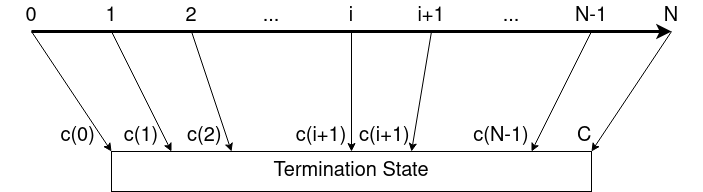
\includegraphics[scale=0.55]{figures/parking_graphic.png}
	\caption{State transitions and costs of the Parking Problem}
\end{figure}

\begin{itemize}
	\item $N$: Number of parking spaces
	\item $p(i)$: Probability that parking space $i$ is free
	\item $c(i)$: Cost of the parking space $i$
	\item $C$: Cost of the garage
\end{itemize}
This problem gives us a total of $2N+1$ states as for each parking place, we need one state for the place being free and one for being taken. We also need an end state indicating that the driver has parked. 

This problem is stochastic as it is uncertain what the next state will be after a transition. For simplicity, we will assume a constant $p$, but the following solutions can also be expanded to handle a function $p(i)$.

\section{Practical Example}
\label{sec:practical}
We will now look at concrete values to compare different approaches to solving the stochastic Markov Decision Process with the following parameters.

The probability of a parking space being free will be constant. The cost function will increase linearly with the space index. We will set the garage cost to half of the number of spaces.
\begin{itemize}
	\item $p(i) = p$
	\item $c(i) = N-i$
	\item $C = \frac{N}{2}$
\end{itemize}

As the cost function is linear and $c(0) > C > c(N)$, we can already expect that the best policy will be to drive up until a certain point and then park at the next free space. Therefore the policy will take the action drive for all states before this threshold and then changes to park at reaching the threshold space.

\begin{figure}[htp]
	\label{figure}
	\centering
	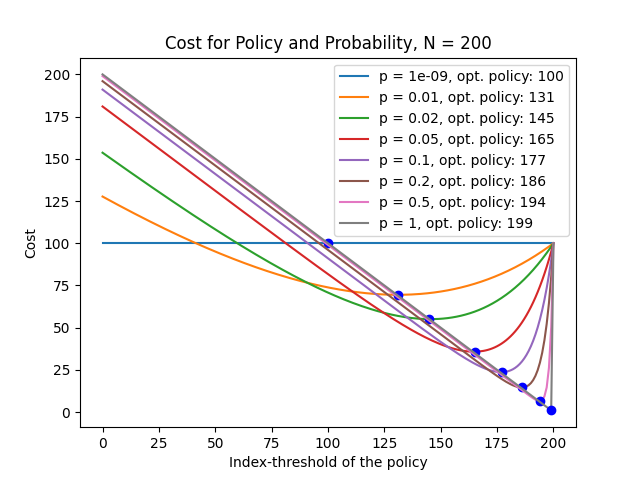
\includegraphics[scale=0.6]{figures/code_statistics/strategy_probabilities_200.png}
	\caption{Cost of per policy and probability for the parking problem}
\end{figure}
We can note from this figure \ref{figure} that the optimal policies and, therefore, costs are linearly dependent on the constant probability of a parking space being free. The expected result if all places are free is to park at the last possible index. If nearly every place is taken, the best policy is to try parking at space $\frac{N}{2}$ as this is at most as bad as parking in the garage.


\subsection{Dynamic Programming Approach}
\label{subsec:dp_approach}
As the entirety of the model is given, we can easily set up an analytical solution using Bells equation \ref{eqn:sto_bellman}. It is crucial to notice that the value of a state does not depend on whether the previous place was free or taken. It depends only on the current index and already considers that this place is possibly taken.

The maximum from the 2 possible actions can be simplified as one already translates to the terminal state ending the recursion. We use $\gamma = 1$ as this gives the optimal solution regarding fully weighted future costs. 

\subsubsection{Recursive Value Function}
\begin{equation*}
	\begin{split}
		&V(N) = C = \frac{N}{2}\\
		&V(i) = p(i) \cdot c(i) + (1-p(i)) \cdot V(i+1)\\
		&0 \leq i < N 
	\end{split}
\end{equation*}

\subsubsection{Explicit Value Function}
\begin{equation}
	\begin{split}
		&V(i) = C \cdot (1-p)^{N-i} + \sum_{j=0}^{N-i} p \cdot (N-i-j) \cdot (1-p)^{j}
	\end{split}
\end{equation}


Now that we have calculated the optimal cost using the entire model, we will approximate this solution using Q-Learning, a model-free algorithm.

\subsection{Q-Learning Approach}
\label{subsec:ql_approach}
Q-Learning does not need to know any probabilities or state transitions. However, it will learn to take actions that will approximate the optimal cost arbitrarily close given enough training steps. 

Therefore the remaining model parameters we need to know are all states, possible actions, and the reward from transitions.

\subsubsection{Reward Function}
Q-Learning tries to maximize the reward in contrast to Dynamic Programming, which minimizes the cost. Therefore we need to transform our cost function into a corresponding reward function. 
We negate the cost function and garage cost \ref{sec:practical} and, as Q-Learning needs positive numbers, level the reward function and garage reward to be all positive by adding $N$.

\begin{itemize}
	\item $C \rightarrow R = \frac{N}{2}$
	\item $c(i) \rightarrow r(i) = i$
\end{itemize}

This function only rewards taking the action to park. We can instead reward transitions and give iterative rewards. It needs to hold that the sum of rewards received upon parking in any space stays equal. However, rewarding actions directly improves the performance of the Q-learning algorithm. An equally performative policy can be trained with fewer iterations than by rewarding the parking action. The following incremental reward function reduces the necessary iterations in learning to less than half of the aggregated reward function above.

\begin{itemize}
	\item Reward from driving forward: $r(i+1) - r(i) = 1$
	\item Reward from transitioning to the garage: $-\frac{N}{2}$
\end{itemize}

\subsubsection{Parameters}
These parameters work well with both reward functions
\begin{itemize}
	\item $\alpha_0 = 0.05$
	\item $\gamma = 0.999$
	\item $\epsilon_0 = 0.05$ 
\end{itemize}
To improve convergence speed, we use a descending learning rate $\alpha_i$ and exploration rate $\epsilon_i$. With $i$ being the current iteration and $n$ being the number of overall iterations.
\begin{itemize}
	\item $\alpha_i = \alpha_0 \frac{n - i + 1}{n}$
	\item $\epsilon_i = \epsilon_0 \frac{n - i + 1}{n}$
\end{itemize}
\subsubsection{Learning Progress}
For space sizes larger than $500$ the learning rate can be increased while keeping the learning stable. Depending on the space size, the number of iterations also needs to be increased.
For $N=200$ and $p = 0.05$ it is enough to have $60000$ learning iterations for stable results.

Using incremental rewards and diminishing learning and exploration rate, the algorithm converges at about $40000$ training iterations. The plotted cost estimates are averaged from $20000$ samples using the current Q-Table policy.

\begin{figure}[htp]
	\centering
	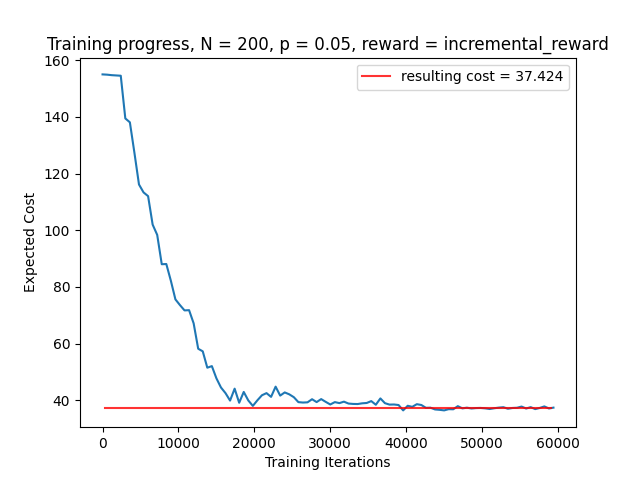
\includegraphics[scale=0.6]{figures/code_statistics/q_training_progress_200.png}
	\caption{Training Progress of Q-Learning Problem, $\alpha_0 = 0.05$, $\epsilon_0 = 0.05$, $\gamma = 0.999$}
\end{figure}

\FloatBarrier

\subsubsection{Results}
Q-Learning can approximate the Dynamic Programming solution quite well. The solution could be better approximated by using a better reward function, tuning the parameters, and increasing the training cycles.
These results use the incremental reward function, a linearly descending learning and exploration rate.

\begin{center}
	\begin{tabular}{ |c|c|c|c| } 
		\hline
		N& \multicolumn{2}{c|}{Q-learning} & Dynamic Programming\\ 
		\hline
		-& mean & standard deviation & -\\ 
		\hline
		$50$ & $17.005$ & $0.263$ & $16.366$ \\ 
		\hline
		$100$ & $26.251$ & $0.519$ & $25.140$ \\ 
		\hline
		$200$ & $37.145$ & $0.989$ & $35.764$ \\ 
		\hline
		$500$ & $53.973$ & $1.591$ & $51.663$ \\ 
		\hline	
	\end{tabular}\\
\end{center}

The results for Q-learning are calculated from 20 learning results, each parking space randomly free with a probability of $0.05$.
        

\chapter{Discussion}
\label{cha:discussion}

In this paper, we discussed the basic theory for optimal control. We listed the requirements and how to define a system to describe the problem accurately. Further, we explained two highly established approaches to solving such a control problem: Dynamic programming and reinforcement learning as respective model-free and model-based methods.

We applied Stochastic Dynamic Programming and Q-Learning to an example and solved the optimal control problem with both methods. Our experimental results align with existing theory and further support that either method is valid in approaching such a problem.

Both methods differ in their advantages and disadvantages. Dynamic programming produces an optimal solution but has high prerequisites. Moreover, the solution on a particular system may not work for a slightly changed model. Model-free reinforcement learning solutions can approximate the solution arbitrarily well. They can also be more general in their solution and therefore applied to model variations. For example, the Q-learning application from the Example \ref{cha:example} works on any given probability distribution $p(i)$. However, the dynamic programming solution can only be applied to a constant $p$.

\section{Future Work}
\label{sec:future_work}

The methods are still active research fields, and this work can be expanded upon in the future. One open question is the effects of a non-constant probability of parking spaces being free or not. 
A more general interest would be to apply a hybrid approach by combining dynamic programming with reinforcement learning to cancel out the disadvantages of both methods.

      
        
\printbibliography             

%%%% end{document}
\end{document}